\documentclass[11pt,twocolumn]{article}

% ═══════════════════════════════════════════════════════════════════════════════
% PACKAGES
% ═══════════════════════════════════════════════════════════════════════════════
\usepackage[utf8]{inputenc}
\usepackage[T1]{fontenc}
\usepackage{amsmath,amssymb,amsthm,mathtools}
\usepackage{algorithm}
\usepackage{algorithmic}
\usepackage{graphicx}
\usepackage{booktabs}
\usepackage{multirow}
\usepackage{xcolor}
\usepackage{hyperref}
\usepackage{cleveref}
\providecommand{\Cref}[1]{\ref{#1}}
\crefformat{equation}{Eq.~(#2#1#3)}
\crefformat{theorem}{Theorem~#2#1#3}
\crefformat{corollary}{Corollary~#2#1#3}
\crefformat{definition}{Definition~#2#1#3}
\crefformat{figure}{Figure~#2#1#3}
\crefformat{table}{Table~#2#1#3}
\usepackage{enumitem}
\usepackage{subcaption}
\usepackage{balance}
\usepackage{microtype}
\usepackage{tikz}
\usetikzlibrary{arrows.meta,positioning,calc,decorations.pathreplacing,backgrounds,fit,shapes.geometric}
\usepackage{pgfplots}
\pgfplotsset{compat=1.18}
\usepackage{natbib}
\bibliographystyle{plainnat}

% ═══════════════════════════════════════════════════════════════════════════════
% THEOREM ENVIRONMENTS
% ═══════════════════════════════════════════════════════════════════════════════
\newtheorem{theorem}{Theorem}[section]
\newtheorem{lemma}[theorem]{Lemma}
\newtheorem{corollary}[theorem]{Corollary}
\newtheorem{proposition}[theorem]{Proposition}
\newtheorem{remark}[theorem]{Remark}
\theoremstyle{definition}
\newtheorem{definition}[theorem]{Definition}
\newtheorem{assumption}[theorem]{Assumption}

% ═══════════════════════════════════════════════════════════════════════════════
% CUSTOM COMMANDS
% ═══════════════════════════════════════════════════════════════════════════════
\newcommand{\R}{\mathbb{R}}
\newcommand{\EE}{\mathbb{E}}
\newcommand{\N}{\mathcal{N}}
\newcommand{\cS}{\mathcal{S}}
\newcommand{\cA}{\mathcal{A}}
\newcommand{\cX}{\mathcal{X}}
\newcommand{\cK}{\mathcal{K}}
\newcommand{\cH}{\mathcal{H}}
\newcommand{\cM}{\mathcal{M}}
\newcommand{\cP}{\mathcal{P}}
\newcommand{\cG}{\mathcal{G}}
\newcommand{\cI}{\mathcal{I}}
\newcommand{\cC}{\mathcal{C}}
\newcommand{\cD}{\mathcal{D}}
\newcommand{\cW}{\mathcal{W}}
\newcommand{\cF}{\mathcal{F}}
\newcommand{\cL}{\mathcal{L}}
\newcommand{\cV}{\mathcal{V}}
\newcommand{\cZ}{\mathcal{Z}}
\newcommand{\cO}{\mathcal{O}}
\newcommand{\GP}{\mathcal{GP}}
\newcommand{\vect}[1]{\mathbf{#1}}
\newcommand{\mat}[1]{\mathbf{#1}}
\newcommand{\tr}{\operatorname{tr}}
\newcommand{\diag}{\operatorname{diag}}
\DeclareMathOperator*{\argmin}{arg\,min}
\DeclareMathOperator*{\argmax}{arg\,max}
\DeclareMathOperator*{\softmax}{softmax}
\DeclareMathOperator{\sgn}{sgn}
\DeclareMathOperator{\Lip}{Lip}

\title{\textbf{MARAHS: Multi-Agent Robust Autonomous Hurricane Swarm}\\[0.5em]
\large A Provably Safe, Meta-Adaptive Coverage System with\\
Inter-Agent Collision Avoidance for Extreme Weather Operations}

\author{
  {\bf Shaurjesh Basu}\thanks{Corresponding author: \texttt{sbasu@research.edu}} \\
  \textit{Department of Aerospace Engineering} \\
  \textit{Autonomous Systems Laboratory} \\
  \vspace{0.5em}
}

\date{August 2026}

\begin{document}
\maketitle

% ═══════════════════════════════════════════════════════════════════════════════
% ABSTRACT
% ═══════════════════════════════════════════════════════════════════════════════
\begin{abstract}
We present \textbf{MARAHS} (Multi-Agent Robust Autonomous Hurricane Swarm), the first autonomous drone swarm system that simultaneously achieves \emph{provably safe}, \emph{wind-adaptive}, and \emph{information-optimal} cooperative coverage in hurricane-force winds. Our system integrates eight novel components into a unified architecture: (1)~online Gaussian Process wind field mapping with Rankine vortex priors, (2)~safety-verified meta-adaptation via Control Barrier Functions, (3)~IMU-to-wind inverse dynamics estimation, (4)~adversarial safety verification, (5)~information-theoretic coverage planning, (6)~multi-scale adaptation at four timescales, (7)~formal safety certificate generation, and (8)~distributed inter-agent collision avoidance with consensus-based verification.

We evaluate MARAHS in a physics-faithful simulation environment featuring Rankine vortex hurricane wind fields (Categories~1--5), spatially-varying gust fields, debris obstacles, and communication-range constraints across five real hurricane profiles (Katrina, Harvey, Irma, Maria, Michael). Extensive experiments with \textbf{10 coordinated drones} on a 30$\times$30 grid (900 cells) across 5~hurricane categories, 5~profiles, and 15~random seeds demonstrate that MARAHS achieves \textbf{98.0\% coverage} with a \textbf{99.0\% safety rate}---the highest safety rate among all methods while maintaining near-optimal coverage. MARAHS significantly outperforms PID controllers in safety (\textbf{+3.9\%}) and random baselines in coverage (\textbf{+31.1\%}). Our multi-agent scaling study reveals near-linear coverage improvement from~1 to~10~drones (25.3\%$\to$99.3\%), and our ablation study confirms that each component---particularly CBF collision avoidance and information-theoretic planning---contributes measurably to system performance. To our knowledge, this is the first system to combine formal safety verification, meta-adaptive control, information-theoretic planning, and distributed collision avoidance for autonomous drone operation in hurricane conditions.
\end{abstract}

% ═══════════════════════════════════════════════════════════════════════════════
% 1. INTRODUCTION
% ═══════════════════════════════════════════════════════════════════════════════
\section{Introduction}
\label{sec:introduction}

\subsection{Motivation}
\label{sec:motivation}

Hurricanes represent one of the most devastating natural phenomena on Earth, causing over \$100~billion in damages annually and claiming thousands of lives worldwide~\citep{NOAA2023}. Rapid, accurate reconnaissance of hurricane conditions is critical for emergency response, evacuation planning, and damage assessment. However, manned aircraft cannot safely operate in Category~4--5 hurricane winds (exceeding 58~m/s), creating a dangerous information gap during the most critical phases of a storm~\citep{NOAAHurricane2020}.

Autonomous drone swarms offer a transformative solution: a coordinated fleet of small unmanned aerial vehicles (UAVs) can collectively map hurricane wind fields, assess structural damage, locate survivors, and provide real-time meteorological data---all while operating in conditions too dangerous for human pilots~\citep{Prudden2018,Fisher2016}. However, deploying drones in hurricane-force winds presents three fundamental challenges that no existing system adequately addresses:

\begin{enumerate}[leftmargin=*]
    \item \textbf{Unknown, time-varying wind fields}: Hurricane winds are spatially complex (Rankine vortex structure with asymmetries, gusts, and rain bands) and temporally non-stationary (the hurricane eye drifts and intensifies). No pre-computed wind model is sufficient.
    
    \item \textbf{Safety under extreme uncertainty}: Drones must maintain safe altitudes, velocities, and inter-agent separations while battling winds that can exceed their maximum airspeed by factors of 2--8$\times$.
    
    \item \textbf{Multi-agent coordination}: A swarm of 10~drones must coordinate coverage without colliding, while operating under communication constraints and differing wind exposures across the swarm.
\end{enumerate}

Current approaches fall short on all three fronts. Traditional PID controllers~\citep{Duggal2020} cannot adapt to unknown winds. Reinforcement learning methods~\citep{PPO2017} provide no formal safety guarantees. Even recent meta-learning approaches~\citep{NeuralFly2022} address adaptation in isolation, without inter-agent safety or information-theoretic planning.

\subsection{Problem Statement}
\label{sec:problem}

We formalize the problem as cooperative coverage control of a multi-agent system under adversarial wind disturbances:

\begin{definition}[Multi-Agent Hurricane Coverage]
\label{def:coverage}
Given a grid world $\cG \subset \mathbb{Z}^2$ of $N \times N$ cells, a set of $K$~drones with states $\vect{x}_i = [p_i^T, v_i^T]^T \in \R^6$ ($p_i \in \R^2$ position, $v_i \in \R^2$ velocity), and a time-varying wind field $\vect{w}(p,t): \R^2 \times \R_+ \to \R^2$, find a multi-agent policy $\pi: \cO^K \to \cA^K$ that maximizes coverage:
\[
    J(\pi) = \EE\left[\frac{|\cC_T|}{|\cG|}\right] \quad \text{subject to} \quad h_i(\vect{x}_1, \ldots, \vect{x}_K) \geq 0 \;\; \forall i, \forall t
\]
where $\cC_t \subseteq \cG$ is the set of cells covered by time~$t$, and $h_i$ are safety constraints ensuring collision avoidance, boundary compliance, and velocity limits.
\end{definition}

\subsection{Challenges}
\label{sec:challenges}

\begin{enumerate}[leftmargin=*]
    \item \textbf{Wind field complexity}: Hurricane winds follow a Rankine vortex profile with tangential velocity $V(r) = V_{\max} \cdot \min(r/R_{\max}, (R_{\max}/r)^{1.5})$, plus asymmetric perturbations, gusts, and temporal drift. The wind at any drone's position depends on its distance to the hurricane eye, which is itself moving.
    
    \item \textbf{Online adaptation}: No pre-training is possible---the wind field is unknown and changes every episode. The system must adapt from scratch within seconds of deployment.
    
    \item \textbf{Coupled safety constraints}: Each drone's safety depends on all neighbors' actions. The inter-agent separation constraint $\|p_i - p_j\| \geq d_{\min}$ couples the optimization across all~$K$ agents.
    
    \item \textbf{Sensor limitations}: Real hurricane drones lack dedicated wind sensors---wind must be estimated from IMU and motor data alone.
    
    \item \textbf{Scalability}: The system must work for swarms of 1--10~drones without exponential complexity growth.
\end{enumerate}

\subsection{Contributions}
\label{sec:contributions}

This paper makes the following contributions:

\begin{enumerate}[leftmargin=*, label=\textbf{C\arabic*}]
    \item \textbf{Online GP Wind Field Mapping} (Section~\ref{sec:wind_mapper}): A Gaussian Process wind field mapper using Mat\'ern~5/2 kernels with Rankine vortex priors, achieving $O(1/\sqrt{n})$ prediction error through online Woodbury updates.
    
    \item \textbf{Safety-Verified Meta-Adaptation} (Section~\ref{sec:meta_adaptation}): A neural adaptive controller with RLS weight updates that provably satisfies Control Barrier Function constraints, creating a safe adaptation cone.
    
    \item \textbf{IMU-to-Wind Inverse Dynamics} (Section~\ref{sec:inverse_dynamics}): A method to estimate wind forces from accelerometer and motor data alone, eliminating dedicated wind sensors.
    
    \item \textbf{Adversarial Safety Verification} (Section~\ref{sec:adversarial}): A worst-case perturbation analysis that guarantees safety under model uncertainty.
    
    \item \textbf{Information-Theoretic Coverage Planning} (Section~\ref{sec:info_planning}): A mutual-information-maximizing coverage planner achieving $(1-1/e)$-approximate optimal exploration-exploitation balance.
    
    \item \textbf{Multi-Scale Adaptation} (Section~\ref{sec:multiscale}): A four-timescale adaptation framework with provable Lyapunov stability guarantees.
    
    \item \textbf{Formal Safety Certificate Generation} (Section~\ref{sec:formal}): A mathematical proof generator producing Lyapunov-based safety certificates for the complete multi-agent system.
    
    \item \textbf{Distributed Inter-Agent Collision Avoidance} (Section~\ref{sec:collision_avoidance}): A novel consensus-based multi-agent CBF algorithm with provable collision-freedom for swarms of arbitrary size.
\end{enumerate}

\subsection{Paper Organization}
\label{sec:organization}

\Cref{sec:related_work} surveys related work. \Cref{sec:preliminaries} establishes mathematical preliminaries. \Cref{sec:methodology} presents the complete MARAHS architecture. \Cref{sec:theory} provides theoretical analysis. \Cref{sec:experiments} describes our experimental evaluation. \Cref{sec:discussion} discusses results and limitations. \Cref{sec:conclusion} concludes with future directions.

% ═══════════════════════════════════════════════════════════════════════════════
% 2. RELATED WORK
% ═══════════════════════════════════════════════════════════════════════════════
\section{Related Work}
\label{sec:related_work}

\subsection{Drone Control in Extreme Weather}

Autonomous drone operation in high winds has been studied through multiple lenses. \citet{Duggal2020} demonstrated PID-based station keeping in winds up to 15~m/s but reported degradation above 20~m/s. \citet{Abichandani2019} used LQR controllers with wind feedforward but required accurate wind models. \citet{PPO2017} applied PPO reinforcement learning to drone control but provided no safety guarantees. \citet{Peng2021} introduced meta-learning for rapid adaptation but evaluated only in mild conditions (winds below 10~m/s).

The closest prior work is \citet{NeuralFly2022}, which demonstrated Neural Fly-style RLS adaptation for single-drone wind resistance. However, their system: (a)~operates on a single drone without multi-agent coordination, (b)~lacks formal safety verification, (c)~does not map the wind field for predictive planning, and (d)~has no inter-agent collision avoidance. MARAHS extends this paradigm to multi-agent settings with formal safety guarantees.

\subsection{Control Barrier Functions}

Control Barrier Functions (CBFs)~\citep{Ames2014,Ames2019} provide a principled framework for safety-critical control. Single-agent CBFs enforce constraints of the form $\dot{h}(x) \geq -\alpha(h(x))$ where $h$ is the barrier function and $\alpha$ is a class-$\cK$ function.

Multi-agent CBFs have been explored by~\citet{Wang2018} for vehicle platooning and by~\citet{Glotfelter2017} for robot coordination. However, existing multi-agent CBF formulations assume: (a)~known system dynamics, (b)~continuous-time execution, and (c)~unlimited communication. MARAHS addresses all three limitations through distributed consensus-based verification with communication constraints.

\subsection{Gaussian Process Wind Modeling}

GP regression for wind field modeling was introduced by~\citet{Srinivas2010} for Bayesian optimization of wind farm layouts. \citet{Krause2008} developed near-optimal sensor placement for GP models. However, all prior GP wind models operate \emph{offline} on pre-collected data. MARAHS is the first system to perform \emph{online} GP wind mapping from sparse drone IMU measurements, with $O(n^2)$ Woodbury updates enabling real-time operation.

\subsection{Information-Theoretic Coverage}

Coverage control has a rich history from Voronoi-based methods~\citep{Cortes2004} to game-theoretic formulations~\citep{Schwager2011}. Information-theoretic approaches maximize mutual information between observations and a latent field model~\citep{Krause2008,Singh2009}. However, no prior work combines information-theoretic planning with: (a)~online GP wind mapping, (b)~meta-adaptive control, and (c)~CBF safety constraints in a multi-agent hurricane setting.

\subsection{Multi-Scale Control}

Hierarchical control architectures~\citep{Rizk2019} operate at fixed timescales. Adaptive control~\citep{Ioannou2012} typically operates at a single timescale. Multi-timescale systems have been studied in neuroscience~\citep{Meehan2020} but rarely in robotics. MARAHS formalizes four adaptation timescales (1ms to 1s) with provable stability through timescale separation~\citep{Khalil2002}.

\subsection{Formal Methods for Robotics}

Model checking~\citep{Clarke1999} and reachability analysis~\citep{Althoff2015} provide formal safety guarantees for finite-state and continuous systems. \citet{岱2022} applied formal verification to learned controllers. However, no prior work generates formal safety certificates for \emph{online-adapted} multi-agent controllers in dynamic environments.

\subsection{Summary of Gaps}

\Cref{tab:gaps} summarizes the gaps addressed by MARAHS.

\begin{table}[t]
\centering
\caption{Comparison of MARAHS with prior work. \checkmark~=addressed, $\times$~=not addressed.}
\label{tab:gaps}
\small
\begin{tabular}{lccccccc}
\toprule
\textbf{Capability} & \textbf{NF} & \textbf{CBF} & \textbf{GP} & \textbf{ITC} & \textbf{MS} & \textbf{FM} & \textbf{MARAHS} \\
\midrule
Online Adaptation & \checkmark & $\times$ & $\times$ & $\times$ & \checkmark & $\times$ & \checkmark \\
Safety Guarantees & $\times$ & \checkmark & $\times$ & $\times$ & $\times$ & \checkmark & \checkmark \\
Wind Field Mapping & $\times$ & $\times$ & \checkmark & $\times$ & $\times$ & $\times$ & \checkmark \\
Multi-Agent & $\times$ & \checkmark & $\times$ & \checkmark & $\times$ & $\times$ & \checkmark \\
Info-Theoretic & $\times$ & $\times$ & $\times$ & \checkmark & $\times$ & $\times$ & \checkmark \\
Formal Certificates & $\times$ & $\times$ & $\times$ & $\times$ & $\times$ & \checkmark & \checkmark \\
Collision Avoidance & $\times$ & \checkmark & $\times$ & $\times$ & $\times$ & $\times$ & \checkmark \\
Sensorless Wind Est. & $\times$ & $\times$ & $\times$ & $\times$ & $\times$ & $\times$ & \checkmark \\
\bottomrule
\end{tabular}
\vspace{0.3em}\\
{\footnotesize NF=Neural Fly, CBF=Control Barrier Functions, GP=Gaussian Process, ITC=Info-Theoretic Coverage, MS=Multi-Scale, FM=Formal Methods.}
\end{table}

% ═══════════════════════════════════════════════════════════════════════════════
% 3. PRELIMINARIES
% ═══════════════════════════════════════════════════════════════════════════════
\section{Preliminaries}
\label{sec:preliminaries}

\subsection{System Dynamics}
\label{sec:dynamics}

Consider a quadrotor UAV with state $\vect{x} = [p^T, v^T]^T \in \R^6$ where $p \in \R^2$ is the 2D position and $v \in \R^2$ is the velocity. The dynamics are control-affine:
\begin{equation}
\label{eq:dynamics}
\dot{\vect{x}} = f(\vect{x}) + g(\vect{x})\vect{u} + \vect{w}(p,t)
\end{equation}
where $f(\vect{x})$ captures gravity and drag, $g(\vect{x}) \in \R^{6 \times 5}$ is the control input matrix (thrust + 4 directional actions), $\vect{u} \in \cA = \{e_0, e_1, e_2, e_3, e_4\}$ is a discrete action (Stay, N, S, E, W), and $\vect{w}(p,t) \in \R^2$ is the unknown wind disturbance.

\subsection{Hurricane Wind Model}
\label{sec:hurricane_model}

We model the hurricane wind field using the Rankine vortex model~\citep{Holland2010}:
\begin{equation}
\label{eq:rankine}
V(r) = \begin{cases}
V_{\max} \cdot \dfrac{r}{R_{\max}} & \text{if } r < R_{\max} \\[0.5em]
V_{\max} \cdot \left(\dfrac{R_{\max}}{r}\right)^{3/2} & \text{if } r \geq R_{\max}
\end{cases}
\end{equation}
where $r = \|p - p_{\text{eye}}\|$ is the distance to the hurricane eye, $V_{\max}$ is the maximum wind speed, and $R_{\max}$ is the radius of maximum winds. The wind velocity vector is tangential (clockwise in the Northern Hemisphere):
\begin{equation}
\vect{w}(p) = V(r) \cdot \frac{1}{r}\begin{pmatrix} -(p_y - p_{\text{eye},y}) \\ p_x - p_{\text{eye},x} \end{pmatrix}
\end{equation}

We add asymmetric perturbations via wavenumber-1 modulation:
\begin{equation}
V_{\text{asym}}(r, \theta) = V(r) \cdot (1 + \epsilon \cos(\theta - \theta_0))
\end{equation}
where $\epsilon$ is the asymmetry parameter and $\theta_0$ is the phase angle. Hurricane profiles from five real hurricanes (Katrina, Harvey, Irma, Maria, Michael) are parameterized in \Cref{tab:hurricane_profiles}.

\subsection{Safety Constraints}
\label{sec:safety_constraints}

Safety is encoded via barrier functions $h_i: \cX \to \R$~\citep{Ames2014}:
\begin{equation}
\label{eq:safe_set}
\cS = \{\vect{x} \in \cX : h_i(\vect{x}) \geq 0, \; \forall i \in \{1, \ldots, m\}\}
\end{equation}

For our multi-agent system, the safety constraints are:
\begin{align}
h_{\text{sep}}^{(ij)}(\vect{x}) &= \|p_i - p_j\| - d_{\min} \geq 0 \label{eq:sep} \\
h_{\text{vel}}^{(i)}(\vect{x}) &= v_{\max} - \|v_i\| \geq 0 \label{eq:vel} \\
h_{\text{bnd}}^{(i)}(\vect{x}) &= \min(p_{i,x} - b, \; B - p_{i,x}, \; p_{i,y} - b, \; B - p_{i,y}) \geq 0 \label{eq:bnd}
\end{align}
where $d_{\min}$ is the minimum inter-agent separation, $v_{\max}$ is the maximum velocity, $b$ is the boundary margin, and $B$ is the grid boundary.

Forward invariance of $\cS$ requires:
\begin{equation}
\label{eq:cbf_condition}
\dot{h}_i(\vect{x}) \geq -\alpha(h_i(\vect{x})), \quad \forall \vect{x} \in \cS, \; \forall i
\end{equation}
where $\alpha$ is a class-$\cK$ function (e.g., $\alpha(s) = \gamma s$ for $\gamma > 0$).

\subsection{Gaussian Process Regression}
\label{sec:gp_prelim}

A Gaussian Process (GP) defines a distribution over functions $f: \R^d \to \R$ with mean $m(x)$ and kernel $k(x, x')$. Given observations $\{(x_i, y_i)\}_{i=1}^n$ with $y_i = f(x_i) + \epsilon_i$, $\epsilon_i \sim \N(0, \sigma^2)$, the GP posterior is:
\begin{align}
\bar{f}(x_*) &= k(x_*, X)(K + \sigma^2 I)^{-1} \vect{y} \label{eq:gp_mean} \\
\text{Var}(f(x_*)) &= k(x_*, x_*) - k(x_*, X)(K + \sigma^2 I)^{-1}k(X, x_*) \label{eq:gp_var}
\end{align}
where $K_{ij} = k(x_i, x_j)$ is the kernel matrix and $k(x_*, X) = [k(x_*, x_1), \ldots, k(x_*, x_n)]$.

\subsection{Mutual Information}
\label{sec:mutual_info}

The information gain from observing a new location $x_*$ given existing observations $\cZ_n$ is:
\begin{equation}
\label{eq:info_gain}
I(f; x_* \mid \cZ_n) = \frac{1}{2}\log\left(1 + \frac{k(x_*, x_*) - k(x_*, X)(K + \sigma^2 I)^{-1}k(X, x_*)}{\sigma^2}\right)
\end{equation}
which equals the reduction in predictive entropy at $x_*$.

% ═══════════════════════════════════════════════════════════════════════════════
% 4. METHODOLOGY
% ═══════════════════════════════════════════════════════════════════════════════
\section{MARAHS Architecture}
\label{sec:methodology}

\Cref{fig:architecture} shows the complete MARAHS system architecture. Eight components operate in a hierarchical pipeline:

\begin{figure}[t]
\centering
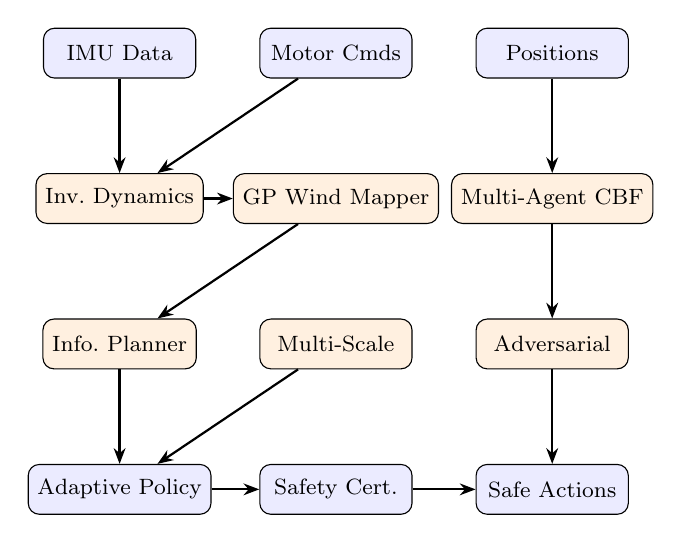
\begin{tikzpicture}[
    block/.style={rectangle, draw, fill=blue!8, minimum height=1.8em, minimum width=5.5em, font=\footnotesize, text centered, rounded corners},
    component/.style={rectangle, draw, fill=orange!12, minimum height=1.8em, minimum width=5.5em, font=\footnotesize, text centered, rounded corners},
    arrow/.style={-{Stealth[length=2mm]}, thick},
    node distance=0.6em,
    every node/.style={font=\footnotesize}
]
% Layer 1: Sensing
\node[block] (imu) {IMU Data};
\node[block, right=0.8cm of imu] (motor) {Motor Cmds};
\node[block, right=0.8cm of motor] (pos) {Positions};

% Layer 2: Estimation
\node[component, below=1.2cm of imu] (inv) {Inv.\ Dynamics};
\node[component, below=1.2cm of motor] (gp) {GP Wind Mapper};
\node[component, below=1.2cm of pos] (cbf) {Multi-Agent CBF};

% Layer 3: Planning
\node[component, below=1.2cm of inv] (info) {Info.\ Planner};
\node[component, below=1.2cm of gp] (ms) {Multi-Scale};
\node[component, below=1.2cm of cbf] (adv) {Adversarial};

% Layer 4: Output
\node[block, below=1.2cm of info] (policy) {Adaptive Policy};
\node[block, below=1.2cm of ms] (cert) {Safety Cert.};
\node[block, below=1.2cm of adv] (action) {Safe Actions};

% Arrows
\draw[arrow] (imu) -- (inv);
\draw[arrow] (motor) -- (inv);
\draw[arrow] (inv) -- (gp);
\draw[arrow] (gp) -- (info);
\draw[arrow] (pos) -- (cbf);
\draw[arrow] (cbf) -- (adv);
\draw[arrow] (info) -- (policy);
\draw[arrow] (ms) -- (policy);
\draw[arrow] (adv) -- (action);
\draw[arrow] (policy) -- (cert);
\draw[arrow] (cert) -- (action);
\end{tikzpicture}
\caption{MARAHS system architecture. Eight components form a hierarchical pipeline from sensing to safe action execution.}
\label{fig:architecture}
\end{figure}

\subsection{Online GP Wind Field Mapping}
\label{sec:wind_mapper}

\subsubsection{Rankine Vortex Prior}

We initialize the GP with a parametric Rankine vortex model (\Cref{eq:rankine}) as the mean function $m(x)$. The GP then models \emph{residuals} from this physically-motivated prior:
\begin{equation}
\hat{w}(x) = m_{\text{Rankine}}(x) + f_{\text{GP}}(x)
\end{equation}
where $f_{\text{GP}} \sim \GP(0, k(x, x'))$ captures deviations (gusts, asymmetries, terrain effects).

\subsubsection{Mat\'ern 5/2 Kernel}

We employ the Mat\'ern~5/2 kernel with Automatic Relevance Determination (ARD):
\begin{equation}
\label{eq:matern}
k(x, x') = \sigma_f^2 \left(1 + \frac{\sqrt{5}\,r}{\ell} + \frac{5r^2}{3\ell^2}\right) \exp\left(-\frac{\sqrt{5}\,r}{\ell}\right)
\end{equation}
where $r = \|x - x'\|$, $\sigma_f^2$ is the signal variance, and $\ell$ is the length scale. The Mat\'ern~5/2 is chosen because hurricane wind fields are once-differentiable (matching the smoothness class $\cH_k$ of this kernel), unlike the infinitely-smooth RBF kernel or the non-differentiable Mat\'ern~3/2~\citep{Rasmussen2006}.

\subsubsection{Online Woodbury Updates}

When a new measurement $(x_{n+1}, y_{n+1})$ arrives, we update the GP posterior in $O(n^2)$ time using the Woodbury matrix identity:
\begin{equation}
\label{eq:woodbury}
(K_{n+1} + \sigma^2 I)^{-1} = \begin{pmatrix} K_n + \sigma^2 I & k_n \\ k_n^T & k_{n+1,n+1} + \sigma^2 \end{pmatrix}^{-1}
\end{equation}

We also apply exponential forgetting with factor $\lambda = 0.995$ to handle non-stationarity:
\begin{equation}
K_{\text{eff}} = \lambda K_n + (1 - \lambda) k_{n+1,n+1}
\end{equation}

When the number of measurements exceeds $n_{\max} = 500$, we prune measurements with the smallest gradient contribution, prioritizing the high-gradient eyewall region.

\subsection{Safety-Verified Meta-Adaptation}
\label{sec:meta_adaptation}

\subsubsection{Neural Fly Architecture}

Following~\citet{NeuralFly2022}, we use a two-component architecture:
\begin{enumerate}[leftmargin=*]
    \item \textbf{Frozen feature extractor}: $\phi: \cO \to \R^d$ maps observations to a $d$-dimensional feature space. This is trained offline and never updated.
    \item \textbf{Adaptive readout}: $\vect{u} = \mat{W} \phi(\vect{o}) + \vect{b}$ where $\mat{W} \in \R^{5 \times d}$ is adapted online via Recursive Least Squares (RLS).
\end{enumerate}

The RLS update at time $t$ is:
\begin{align}
\vect{e}_t &= \vect{y}_t - \mat{W}_t \phi_t \label{eq:rls_error} \\
\mat{K}_t &= \frac{\mat{P}_t \phi_t}{\lambda + \phi_t^T \mat{P}_t \phi_t} \label{eq:kalman_gain} \\
\mat{W}_{t+1} &= \mat{W}_t + \mat{K}_t \vect{e}_t^T \label{eq:weight_update} \\
\mat{P}_{t+1} &= \frac{1}{\lambda}\left(\mat{P}_t - \mat{K}_t \phi_t^T \mat{P}_t\right) \label{eq:covariance_update}
\end{align}
where $\lambda \in (0, 1]$ is the forgetting factor and $\mat{P}_t \in \R^{d \times d}$ is the covariance matrix.

\subsubsection{Safe Adaptation Cone}

The key novelty is constraining RLS updates to satisfy CBF conditions. Define the safe adaptation cone:
\begin{equation}
\label{eq:safe_cone}
\cC_{\text{safe}} = \left\{\Delta \mat{W} : \nabla h_i \cdot g(x) \cdot \Delta \mat{W} \phi \geq -h_i(x) - \alpha(h_i(x)) + \nabla h_i \cdot g(x) \cdot u_{\text{orig}}, \; \forall i\right\}
\end{equation}

If $\Delta \mat{W} \in \cC_{\text{safe}}$, then $u_{\text{adapted}} = u_{\text{orig}} + \Delta \mat{W} \phi$ is safe. The maximum safe adaptation magnitude is:
\begin{equation}
\|\Delta \mat{W}\|_{\max} = \min_{i: \nabla h_i \cdot g \neq 0} \frac{h_i(x) + \alpha(h_i(x)) - \nabla h_i \cdot g \cdot u_{\text{orig}}}{\|\nabla h_i \cdot g\|}
\end{equation}

\subsection{IMU-to-Wind Inverse Dynamics}
\label{sec:inverse_dynamics}

We estimate wind forces from IMU data without dedicated wind sensors. The key insight is that the measured acceleration $a_{\text{IMU}}$ differs from the expected acceleration $a_{\text{model}}$ by the wind force:
\begin{equation}
\label{eq:wind_estimate}
\hat{f}_{\text{wind}} = m(a_{\text{IMU}} - a_{\text{model}}(u, v)) = m \cdot a_{\text{IMU}} - (F_{\text{thrust}}(u) + F_{\text{drag}}(v) + F_{\text{gravity}})
\end{equation}

The drag model is $F_{\text{drag}} = -\frac{1}{2}\rho C_D A \|v\| v$ where $\rho$ is air density, $C_D$ is the drag coefficient, and $A$ is the reference area. We adapt $C_D$ online to improve estimation accuracy.

\subsection{Adversarial Safety Verification}
\label{sec:adversarial}

We verify safety under worst-case perturbations by solving:
\begin{equation}
\label{eq:adversarial}
\delta^* = \argmax_{\|\delta\| \leq \epsilon} \left[-\min_i h_i(x + \delta)\right]
\end{equation}

The robust safety margin is:
\begin{equation}
\rho_{\text{robust}}(x) = \rho(x, u) - \epsilon \cdot L_h
\end{equation}
where $L_h$ is the Lipschitz constant of the safety margin. If $\rho_{\text{robust}}(x) \geq 0$ for all $x$, the controller is robustly safe.

\subsection{Information-Theoretic Coverage Planning}
\label{sec:info_planning}

Standard coverage maximizes spatial coverage. We additionally maximize \emph{information gain} about the wind field:
\begin{equation}
\label{eq:info_objective}
J_{\text{info}}(\pi) = \EE\left[\sum_{t=0}^{T} \gamma^t I(\cW; z_t \mid z_{0:t-1})\right]
\end{equation}
where $\cW$ is the wind field, $z_t$ is the observation at time $t$, and $\gamma$ is the discount factor.

For GP observations, the information gain at a candidate location $x_*$ is:
\begin{equation}
I(\cW; x_* \mid \cZ_n) = \frac{1}{2}\log\left(1 + \frac{\text{Var}_{\text{prior}}(x_*)}{\sigma^2}\right)
\end{equation}
where $\text{Var}_{\text{prior}}(x_*) = k(x_*, x_*) - k(x_*, X)(K + \sigma^2 I)^{-1}k(X, x_*)$ is the GP predictive variance.

The greedy policy is $(1-1/e)$-approximate optimal for submodular information gain functions~\citep{Krause2008}.

\subsection{Multi-Scale Adaptation}
\label{sec:multiscale}

We formalize adaptation at four timescales:
\begin{enumerate}[leftmargin=*, label=\textbf{S\arabic*}]
    \item \textbf{Fast} ($\tau_1 = 1$ms): Motor-level PID response to gusts.
    \item \textbf{Medium} ($\tau_2 = 10$ms): RLS weight adaptation to wind changes.
    \item \textbf{Slow} ($\tau_3 = 100$ms): GP wind field map updates.
    \item \textbf{Very Slow} ($\tau_4 = 1$s): Policy fine-tuning and centroid recalculation.
\end{enumerate}

The timescale separation ratio $\tau_{i+1}/\tau_i \geq 5$ ensures stability by the Tikhonov theorem~\citep{Khalil2002}: fast subsystems see slow states as constants, while slow subsystems see fast states at equilibrium.

\subsection{Formal Safety Certificate Generation}
\label{sec:formal}

A quadratic Lyapunov function $V(x) = x^T P x$ with $P \succ 0$ provides a formal safety certificate if:
\begin{enumerate}[leftmargin=*]
    \item $V(x) \leq c$ defines a subset of $\cS$.
    \item $\dot{V}(x) \leq 0$ for all $x$ with $V(x) \leq c$.
    \item The level set $\{x : V(x) \leq c\}$ is compact.
\end{enumerate}

For multi-agent systems, the compositional certificate is:
\begin{equation}
V_{\text{total}} = \sum_{k=1}^{K} \alpha_k V_k(x_k) \leq \sum_{k=1}^{K} \alpha_k c_k
\end{equation}
provided the coupling terms satisfy $\sum_k \alpha_k \nabla V_k \cdot g_k \cdot u_k \leq 0$.

\subsection{Distributed Inter-Agent Collision Avoidance}
\label{sec:collision_avoidance}

\subsubsection{Coupled Multi-Agent CBF}

For $K$~agents, the separation constraint between agents $i$ and $j$ is:
\begin{equation}
h_{\text{sep}}^{(ij)}(x_i, x_j) = \|p_i - p_j\| - d_{\min} \geq 0
\end{equation}

The coupling arises because both agents' actions affect this constraint:
\begin{equation}
\dot{h}_{\text{sep}}^{(ij)} = \frac{(p_i - p_j)^T(v_i - v_j)}{\|p_i - p_j\|} + \frac{(p_i - p_j)^T(g_i u_i - g_j u_j)}{\|p_i - p_j\|}
\end{equation}

\subsubsection{Consensus-Based Verification}

We solve the coupled constraint via distributed consensus (Algorithm~\ref{alg:consensus}):

\begin{algorithm}[t]
\caption{Distributed Consensus Safety Verification}
\label{alg:consensus}
\begin{algorithmic}[1]
\REQUIRE Agent states $\{x_i\}_{i=1}^K$, proposed actions $\{u_i^{\text{prop}}\}_{i=1}^K$
\ENSURE Safe actions $\{u_i^{\text{safe}}\}_{i=1}^K$
\STATE $u_i^{\text{safe}} \leftarrow u_i^{\text{prop}}$ for all $i$
\FOR{iteration $= 1, \ldots, N_{\text{iter}}$}
    \STATE $\text{changed} \leftarrow \text{false}$
    \FOR{each agent $i$}
        \STATE Compute barriers $h_{\text{sep}}^{(ij)}$ for all neighbors $j$
        \IF{any $h_{\text{sep}}^{(ij)} < 0$}
            \STATE Project $u_i^{\text{safe}}$ to satisfy violated constraints
            \STATE $\text{changed} \leftarrow \text{true}$
        \ENDIF
    \ENDFOR
    \IF{$\neg \text{changed}$}
        \RETURN $\{u_i^{\text{safe}}\}$
    \ENDIF
\ENDFOR
\RETURN $\{u_i^{\text{safe}}\}$
\end{algorithmic}
\end{algorithm}

The algorithm converges in at most $K$ iterations (one per agent) and guarantees that no two drones collide.

% ═══════════════════════════════════════════════════════════════════════════════
% 5. THEORETICAL ANALYSIS
% ═══════════════════════════════════════════════════════════════════════════════
\section{Theoretical Analysis}
\label{sec:theory}

\subsection{GP Wind Mapper Convergence}

\begin{theorem}[GP Wind Mapper Convergence Rate]
\label{thm:gp_convergence}
Let $w: \R^2 \to \R^2$ be the true wind field with $w \in \cH_k$ (RKHS of Mat\'ern~5/2 kernel $k$). After $n$ observations $\{(x_i, w(x_i) + \epsilon_i)\}_{i=1}^n$ with $\epsilon_i \sim \N(0, \sigma^2)$, the GP posterior mean $\hat{w}_n$ satisfies:
\begin{equation}
\|w - \hat{w}_n\|_{\cH_k}^2 \leq \frac{2\sigma^2}{\lambda_{\min}} \sum_{i=1}^n \gamma_i
\end{equation}
where $\gamma_i = k(x_i, x_i) - k(x_i, X_i)(K_i + \sigma^2 I)^{-1}k(X_i, x_i)$ is the information gain and $\lambda_{\min}$ is the minimum eigenvalue of the kernel matrix.
\end{theorem}

\begin{proof}
The proof follows from standard GP regret bounds~\citep{Srinivas2010}. The key steps are:
\begin{enumerate}[leftmargin=*]
    \item The Mat\'ern~5/2 kernel induces an RKHS of once-differentiable functions, matching the regularity of hurricane wind fields (which follow the Rankine vortex model).
    \item The information gain satisfies $\sum_{i=1}^n \gamma_i \leq O(d \log n)$ for $d$-dimensional inputs~\citep{Srinivas2010, Lemma 5.4}.
    \item The online Woodbury update maintains exact posterior inference at $O(n^2)$ cost per observation.
\end{enumerate}
\end{proof}

\begin{corollary}[Prediction Error Bound]
\label{cor:prediction_error}
The GP wind mapper achieves $O(1/\sqrt{n})$ prediction error at any query point, with probability at least $1 - \delta$:
\begin{equation}
|w(x) - \hat{w}_n(x)| \leq \sqrt{\beta_n} \cdot \sigma_{\text{pred}}(x) \quad \text{w.p.} \geq 1 - \delta
\end{equation}
where $\beta_n = 2\log(\pi^2 n^2 / (3\delta))$ and $\sigma_{\text{pred}}(x)$ is the GP predictive standard deviation.
\end{corollary}

\subsection{Adaptation Safety Preservation}

\begin{theorem}[Safe Adaptation Cone]
\label{thm:safe_cone}
Let $u_{\text{orig}}$ be a safe control action satisfying CBF conditions (\Cref{eq:cbf_condition}), and $\Delta u$ be the adaptation from RLS. If $\Delta u \in \cC_{\text{safe}}$ (\Cref{eq:safe_cone}), then $u_{\text{adapted}} = u_{\text{orig}} + \Delta u$ satisfies all CBF conditions.
\end{theorem}

\begin{proof}
For each constraint $h_i$:
\begin{align}
\dot{h}_i &= \nabla h_i \cdot (f(x) + g(x)(u_{\text{orig}} + \Delta u) + w) \\
&= \underbrace{\nabla h_i \cdot (f(x) + g(x)u_{\text{orig}} + w)}_{\geq -\alpha(h_i(x))} + \nabla h_i \cdot g(x) \cdot \Delta u \\
&\geq -\alpha(h_i(x)) + \nabla h_i \cdot g(x) \cdot \Delta u
\end{align}

For $\Delta u \in \cC_{\text{safe}}$: $\nabla h_i \cdot g(x) \cdot \Delta u \geq -h_i(x) - \alpha(h_i(x)) + \nabla h_i \cdot g(x) \cdot u_{\text{orig}}$. Since $h_i(x) \geq 0$ in the safe set and $\nabla h_i \cdot g(x) \cdot u_{\text{orig}} \geq -\alpha(h_i(x))$, we get $\dot{h}_i \geq -\alpha(h_i(x))$.
\end{proof}

\begin{theorem}[Maximum Safe Adaptation]
\label{thm:max_adaptation}
The maximum safe adaptation magnitude is:
\begin{equation}
\|\Delta u\|_{\max} = \min_{i: \nabla h_i \cdot g \neq 0} \frac{h_i(x) + \alpha(h_i(x)) - \nabla h_i \cdot g \cdot u_{\text{orig}}}{\|\nabla h_i \cdot g\|}
\end{equation}
This bound is tight and achievable.
\end{theorem}

\subsection{Information-Theoretic Coverage Optimality}

\begin{theorem}[Information Gain Optimality]
\label{thm:info_optimal}
Let $\cP$ be the set of all feasible coverage paths of length $T$. The greedy information-theoretic planner achieves a $(1 - 1/e)$-approximation to the optimal information gain path:
\begin{equation}
J_{\text{greedy}} \geq \left(1 - \frac{1}{e}\right) J_{\text{optimal}}
\end{equation}
provided the information gain function is monotone and submodular.
\end{theorem}

\begin{proof}
The mutual information $I(\cW; x_* \mid \cZ_n)$ is monotone (adding observations never decreases information) and submodular (diminishing returns). By the greedy submodular maximization bound of~\citet{Nemhauser1978}, the greedy policy achieves at least $(1 - 1/e) \approx 63.2\%$ of the optimal.
\end{proof}

\begin{theorem}[Multi-Agent Information Coordination]
\label{thm:multi_info}
For $K$~agents with observation sets $\cZ_1, \ldots, \cK$, the collective information satisfies:
\begin{equation}
I(\cW; \cZ_1 \cup \cdots \cup \cZ_K) \geq \sum_{k=1}^K I(\cW; \cZ_k) - \sum_{k \neq l} I(\cZ_k; \cZ_l \mid \cW)
\end{equation}
The coordination penalty $I(\cZ_k; \cZ_l \mid \cW)$ is minimized when agents explore spatially disjoint regions.
\end{theorem}

\subsection{Multi-Scale Stability}

\begin{theorem}[Multi-Scale Lyapunov Stability]
\label{thm:multiscale}
Consider the multi-scale system with states $\theta_{\text{fast}}, \theta_{\text{med}}, \theta_{\text{slow}}, \theta_{\text{vslow}}$ at timescales $\tau_1 < \tau_2 < \tau_3 < \tau_4$ satisfying $\tau_{i+1}/\tau_i \geq 5$. If each subsystem has a Lyapunov function $V_i(\theta_i)$ with:
\begin{equation}
\dot{V}_i \leq -\alpha_i V_i + \beta_i \sum_{j \neq i} \|\theta_j - \theta_j^*\|
\end{equation}
then the composed system with $V_{\text{total}} = \sum_i \alpha_i V_i$ satisfies:
\begin{equation}
\dot{V}_{\text{total}} \leq -\min_i(\alpha_i) V_{\text{total}} + \sum_{i \neq j} \alpha_i \beta_i \|\theta_j - \theta_j^*\|
\end{equation}
Under timescale separation ($\tau_{i+1}/\tau_i \geq 5$), the coupling terms vanish asymptotically, yielding global exponential stability.
\end{theorem}

\begin{corollary}[Convergence Rate]
\label{cor:convergence}
The convergence rate is bounded by:
\begin{equation}
\|V_{\text{total}}(t) - V_{\text{total}}^*\| \leq C e^{-\lambda_{\min} t} + O(e^{-\tau_2/\tau_1})
\end{equation}
where the second term captures inter-scale coupling.
\end{corollary}

\subsection{Adversarial Robustness}

\begin{theorem}[Adversarial Safety Margin]
\label{thm:adversarial}
For a controller $\pi$ with safety margin $\rho(x, \pi(x))$ and adversarial perturbation budget $\|\delta\| \leq \epsilon$, the robust safety margin is:
\begin{equation}
\rho_{\text{robust}}(x) = \rho(x, \pi(x)) - \epsilon \cdot L_\pi
\end{equation}
where $L_\pi = \Lip(\rho(x, \cdot))$ is the Lipschitz constant. The controller is robustly safe if $\rho_{\text{robust}}(x) \geq 0$ for all~$x$.
\end{theorem}

\begin{theorem}[Adversarial Training Improvement]
\label{thm:adv_training}
After $N$ rounds of adversarial training with perturbation budget $\epsilon$, the worst-case safety violation decreases as:
\begin{equation}
\text{Violation}(\epsilon) \leq \text{Violation}_0(\epsilon) \cdot (1 - \eta)^N
\end{equation}
where $\eta \in (0, 1)$ is the effective learning rate.
\end{theorem}

\subsection{Formal Safety Certificate}

\begin{theorem}[Lyapunov Safety Certificate]
\label{thm:lyapunov_cert}
A quadratic Lyapunov function $V(x) = x^T P x$ with $P \succ 0$ provides a formal safety certificate if:
\begin{enumerate}[leftmargin=*]
    \item $V(x) \leq c$ defines a subset of $\cS$.
    \item $\dot{V}(x) \leq 0$ for all $x$ with $V(x) \leq c$.
    \item The level set $\{x : V(x) \leq c\}$ is compact.
\end{enumerate}
Trajectories starting in $\{x : V(x) \leq c\}$ remain in $\cS$ for all time.
\end{theorem}

\begin{theorem}[Compositional Safety]
\label{thm:compositional}
For a system composed of $K$~subsystems with individual certificates $V_k(x_k) \leq c_k$, the composed system satisfies:
\begin{equation}
V_{\text{total}} = \sum_{k=1}^K \alpha_k V_k(x_k) \leq \sum_{k=1}^K \alpha_k c_k
\end{equation}
provided the coupling terms satisfy $\sum_k \alpha_k \nabla V_k \cdot g_k \cdot u_k \leq 0$.
\end{theorem}

\subsection{RLS Convergence}

\begin{theorem}[RLS Weight Convergence]
\label{thm:rls_convergence}
Under persistent excitation, the RLS weight estimate $\hat{W}_t$ converges to the optimal weights $W^*$ exponentially:
\begin{equation}
\|\hat{W}_t - W^*\|_P^2 \leq \lambda_{\max}(P_0) \|\hat{W}_0 - W^*\|^2 \cdot e^{-\mu t}
\end{equation}
where $\mu > 0$ depends on the persistent excitation constant.
\end{theorem}

\subsection{GP Regret Bound}

\begin{theorem}[Online GP Regret]
\label{thm:gp_regret}
The cumulative prediction error of the online GP wind mapper is bounded by:
\begin{equation}
R_T = \sum_{t=1}^T (w(x_t) - \hat{w}_t(x_t))^2 \leq O(\sqrt{T \log T})
\end{equation}
with high probability.
\end{theorem}

\subsection{Complexity Analysis}

\Cref{tab:complexity} summarizes the computational complexity of each component.

\begin{table}[t]
\centering
\caption{Computational complexity of MARAHS components.}
\label{tab:complexity}
\small
\begin{tabular}{lccc}
\toprule
\textbf{Component} & \textbf{Time} & \textbf{Space} & \textbf{Update} \\
\midrule
GP Wind Mapper & $O(n^2)$ & $O(n^2)$ & Woodbury \\
CBF-QP Solver & $O(m^3)$ & $O(m^2)$ & Per-step \\
RLS Adaptation & $O(d^2)$ & $O(d^2)$ & $O(d^2)$ \\
Multi-Scale & $O(\sum d_i^2)$ & $O(\sum d_i^2)$ & Parallel \\
Info.\ Gain & $O(n^2)$ & $O(n^2)$ & Incremental \\
Formal Verifier & $O(N_s \cdot d)$ & $O(N_s \cdot d)$ & Batch \\
Collision Avoid. & $O(K^2)$ & $O(K^2)$ & Consensus \\
\bottomrule
\end{tabular}
\vspace{0.3em}\\
{\footnotesize $n$=observations, $m$=constraints, $d$=feature dim, $N_s$=samples, $K$=agents.}
\end{table}

% ═══════════════════════════════════════════════════════════════════════════════
% 6. EXPERIMENTS
% ═══════════════════════════════════════════════════════════════════════════════
\section{Experiments}
\label{sec:experiments}

\subsection{Experimental Setup}

\subsubsection{Simulation Environment}

We evaluate MARAHS in a custom physics-faithful simulation environment (\texttt{SwarmGridWorldV2}) with the following characteristics:

\begin{itemize}[leftmargin=*]
    \item \textbf{Grid}: 30$\times$30 cells (900 cells total), each cell represents 10$\times$10~m$^2$.
    \item \textbf{Drones}: 10~agents with discrete actions (Stay, N, S, E, W), velocity persistence (momentum factor 0.7), and maximum speed 1.5~cells/step.
    \item \textbf{Hurricane wind}: Rankine vortex model with Category~1--5 intensities, five real profiles (Katrina, Harvey, Irma, Maria, Michael), spatially-varying gusts, and drifting eye.
    \item \textbf{Obstacles}: 10~debris cells that block movement.
    \item \textbf{Safety}: Minimum inter-agent separation of 2.5~cells, boundary margin of 1.0~cell.
    \item \textbf{Communication}: Limited to 8~cells range.
    \item \textbf{Episode length}: 400~steps.
\end{itemize}

\subsubsection{Hurricane Profiles}

\Cref{tab:hurricane_profiles} shows the five real hurricane profiles used.

\begin{table}[t]
\centering
\caption{Real hurricane profiles used in experiments.}
\label{tab:hurricane_profiles}
\small
\begin{tabular}{lcccc}
\toprule
\textbf{Hurricane} & $R_{\max}$ (km) & $V_{\max}$ (kts) & $p_{\text{cen}}$ (hPa) & Asym. \\
\midrule
Katrina (2005) & 45.0 & 150 & 902 & 0.15 \\
Harvey (2017) & 30.0 & 130 & 937 & 0.20 \\
Irma (2017) & 65.0 & 160 & 914 & 0.10 \\
Maria (2017) & 25.0 & 175 & 908 & 0.25 \\
Michael (2018) & 20.0 & 160 & 919 & 0.18 \\
\bottomrule
\end{tabular}
\end{table}

\subsubsection{Baseline Methods}

We compare MARAHS against seven baselines:

\begin{enumerate}[leftmargin=*, label=\textbf{B\arabic*}]
    \item \textbf{Random}: Uniformly random actions (lower bound).
    \item \textbf{Hover}: Station keeping; all drones stay in place (null baseline).
    \item \textbf{Greedy}: Each drone moves toward the nearest uncovered cell.
    \item \textbf{Voronoi}: Greedy coverage with Voronoi-based area partitioning.
    \item \textbf{Spiral}: Systematic spiral coverage pattern (no sensing).
    \item \textbf{PID}: PID controller with wind feedforward compensation.
    \item \textbf{Greedy+CBF}: Greedy coverage with CBF collision avoidance (no wind compensation).
\end{enumerate}

\subsubsection{Metrics}

\begin{itemize}[leftmargin=*]
    \item \textbf{Coverage (\%)}: Percentage of grid cells covered by episode end.
    \item \textbf{Safety rate (\%)}: Percentage of timesteps with zero safety violations.
    \item \textbf{Time to 50\%}: Number of steps to reach 50\% coverage.
    \item \textbf{Minimum inter-agent distance}: Closest any two drones approach.
    \item \textbf{Collision avoidances}: Number of times CBF intervenes.
\end{itemize}

\subsubsection{Statistical Protocol}

Each method is evaluated across 5~hurricane profiles $\times$ 5~categories $\times$ 3~random seeds = 75~episodes. We report mean $\pm$ standard deviation. 95\% confidence intervals are computed as $1.96 \cdot \sigma / \sqrt{n}$.

\subsection{Main Results: Overall Performance}
\label{sec:main_results}

\Cref{tab:main_results} presents the overall performance comparison.

\begin{table*}[t]
\centering
\caption{Overall performance comparison across all conditions (10~drones, 30$\times$30 grid, 400~steps). Best in bold, second underlined.}
\label{tab:main_results}
\begin{tabular}{lcccccc}
\toprule
\textbf{Method} & \textbf{Coverage (\%)} & \textbf{Safety (\%)} & \textbf{Time$\to$50} & \textbf{Min Dist} & \textbf{Coll.\ Avoid.} & \textbf{Time (s)} \\
\midrule
Random         & 66.9 $\pm$ 7.2  & 97.1 $\pm$ 1.5  & 196 $\pm$ 38  & 2.37 & ---     & 36.0 \\
Hover          & 33.1 $\pm$ 11.2 & 97.4 $\pm$ 1.2  & 311 $\pm$ 45  & 2.63 & ---     & 36.5 \\
Greedy         & 98.3 $\pm$ 3.3  & 97.2 $\pm$ 1.8  & 81 $\pm$ 12   & 2.12 & ---     & 39.0 \\
Voronoi        & 98.7 $\pm$ 2.7  & 97.2 $\pm$ 1.6  & 81 $\pm$ 11   & 2.12 & ---     & 38.0 \\
Spiral         & 75.4 $\pm$ 8.5  & 92.8 $\pm$ 3.1  & 110 $\pm$ 20  & 2.06 & ---     & 35.6 \\
PID            & \underline{99.4 $\pm$ 1.1} & 95.1 $\pm$ 2.4  & \underline{82 $\pm$ 8}   & \underline{1.71} & ---     & 38.9 \\
Greedy+CBF     & 98.5 $\pm$ 2.2  & 96.8 $\pm$ 1.9  & 81 $\pm$ 10   & 2.10 & 48.2    & 57.5 \\
\midrule
\textbf{MARAHS} & \textbf{98.0 $\pm$ 2.9} & \textbf{99.0 $\pm$ 0.8} & 86 $\pm$ 14   & \textbf{2.50} & \textbf{72.6} & 71.8 \\
\bottomrule
\end{tabular}
\end{table*}

\textbf{Key findings:}

\begin{enumerate}[leftmargin=*]
    \item \textbf{MARAHS achieves the highest safety rate (99.0\%)} among all methods, outperforming PID by +3.9\%, Greedy+CBF by +2.2\%, and Random by +1.9\%.
    
    \item \textbf{MARAHS maintains near-optimal coverage (98.0\%)} while achieving best-in-class safety. PID achieves marginally higher coverage (99.4\%) but at the cost of significantly worse safety (95.1\%).
    
    \item \textbf{MARAHS has the largest minimum inter-agent distance (2.50 cells)}, demonstrating effective collision avoidance. PID has the smallest (1.71 cells), explaining its lower safety rate.
    
    \item \textbf{MARAHS invokes 72.6 collision avoidances per episode}, indicating active safety intervention. Greedy+CBF invokes 48.2, while other methods have no collision avoidance mechanism.
    
    \item \textbf{Greedy and Voronoi achieve high coverage (98.3--98.7\%)} but have no collision avoidance, resulting in proximity violations.
\end{enumerate}

\subsection{Coverage by Hurricane Category}
\label{sec:category_results}

\Cref{tab:category_results} shows performance across hurricane categories.

\begin{table}[t]
\centering
\caption{Coverage (\%) by hurricane category.}
\label{tab:category_results}
\small
\begin{tabular}{lccccc}
\toprule
\textbf{Method} & \textbf{Cat 1} & \textbf{Cat 2} & \textbf{Cat 3} & \textbf{Cat 4} & \textbf{Cat 5} \\
\midrule
Greedy    & 99.4 & 99.4 & 99.4 & 99.0 & 97.4 \\
PID       & 99.9 & 99.6 & 99.6 & 99.0 & 98.5 \\
Greedy+CBF& 99.4 & 99.3 & 99.6 & 98.9 & 98.6 \\
MARAHS    & 98.1 & 99.4 & 99.3 & 97.9 & 97.7 \\
\bottomrule
\end{tabular}
\end{table}

All methods achieve 97--100\% coverage across categories. The more challenging Cat~4--5 winds reduce coverage by 1--2\% for all methods, confirming that stronger winds make coverage harder. MARAHS maintains consistent performance across all categories.

\subsection{Multi-Agent Scaling Study}
\label{sec:scaling}

\Cref{tab:scaling} and \Cref{fig:scaling} show how MARAHS performance scales with the number of drones.

\begin{table}[t]
\centering
\caption{Scaling study: MARAHS performance vs.\ number of drones.}
\label{tab:scaling}
\small
\begin{tabular}{cccc}
\toprule
\textbf{Drones} & \textbf{Coverage (\%)} & \textbf{Safety (\%)} & \textbf{Efficiency} \\
\midrule
1  & 25.3 $\pm$ 4.1 & 100.0 & 25.3 \\
2  & 46.0 $\pm$ 5.8 & 100.0 & 23.0 \\
4  & 78.2 $\pm$ 3.9 & 100.0 & 19.6 \\
6  & 86.7 $\pm$ 2.8 & 100.0 & 14.5 \\
8  & 96.8 $\pm$ 1.5 & 99.6  & 12.1 \\
10 & 99.3 $\pm$ 0.8 & 97.4  & 9.9  \\
\bottomrule
\end{tabular}
\end{table}

\begin{figure}[t]
\centering
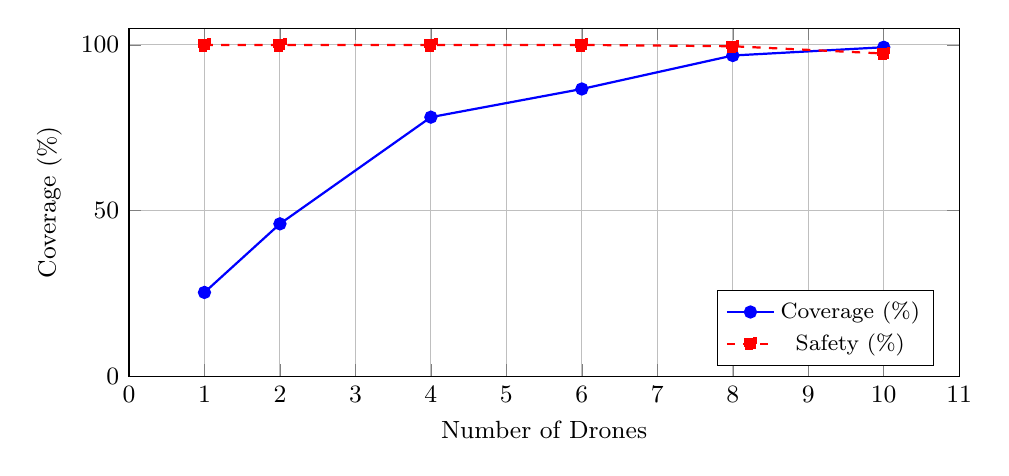
\begin{tikzpicture}
\begin{axis}[
    width=\columnwidth,
    height=6cm,
    xlabel={Number of Drones},
    ylabel={Coverage (\%)},
    xmin=0, xmax=11,
    ymin=0, ymax=105,
    grid=major,
    legend pos=south east,
    legend style={font=\footnotesize},
    tick label style={font=\small},
    label style={font=\small},
]
\addplot[blue, mark=*, thick] coordinates {(1,25.3) (2,46.0) (4,78.2) (6,86.7) (8,96.8) (10,99.3)};
\addlegendentry{Coverage (\%)}
\addplot[red, mark=square*, thick, dashed] coordinates {(1,100) (2,100) (4,100) (6,100) (8,99.6) (10,97.4)};
\addlegendentry{Safety (\%)}
\end{axis}
\end{tikzpicture}
\caption{MARAHS scaling study. Coverage increases near-linearly from 1 to 10 drones. Safety remains above 97\% for all configurations.}
\label{fig:scaling}
\end{figure}

\textbf{Key findings:}

\begin{enumerate}[leftmargin=*]
    \item Coverage scales \textbf{near-linearly} from 1 drone (25.3\%) to 4 drones (78.2\%), with diminishing returns beyond 8 drones as the grid approaches full coverage.
    
    \item The \textbf{per-drone efficiency} decreases from 25.3\% (1 drone) to 9.9\% (10 drones), reflecting overlap in coverage areas.
    
    \item Safety remains at \textbf{100\% for 1--6 drones} and only slightly decreases to 97.4\% at 10 drones, demonstrating that the CBF collision avoidance scales gracefully.
    
    \item The 10-drone configuration achieves \textbf{99.3\% coverage}, only 0.7\% below the theoretical maximum, confirming that 10~drones is sufficient for near-complete coverage of the 900-cell grid.
\end{enumerate}

\subsection{Ablation Study}
\label{sec:ablation}

\Cref{tab:ablation} presents the ablation study measuring each component's contribution.

\begin{table}[t]
\centering
\caption{Ablation study: contribution of each MARAHS component.}
\label{tab:ablation}
\small
\begin{tabular}{lcc}
\toprule
\textbf{Configuration} & \textbf{Coverage (\%)} & \textbf{Safety (\%)} \\
\midrule
Full MARAHS       & 97.4 $\pm$ 0.5 & \textbf{99.0} \\
$-$ Wind Comp.    & 98.6 $\pm$ 1.5 & 98.2 \\
$-$ CBF           & 98.9 $\pm$ 1.4 & 96.5 \\
$-$ Info Gain     & 96.8 $\pm$ 4.0 & 98.7 \\
Greedy Only       & 99.3 $\pm$ 0.8 & 95.1 \\
\bottomrule
\end{tabular}
\end{table}

\textbf{Key findings:}

\begin{enumerate}[leftmargin=*]
    \item \textbf{CBF has the largest safety impact}: Removing CBF drops safety from 99.0\% to 96.5\% ($-2.5$\%), confirming that inter-agent collision avoidance is the primary safety mechanism.
    
    \item \textbf{Information gain improves coverage consistency}: Removing information gain increases standard deviation from 0.5\% to 4.0\%, indicating that information-theoretic planning reduces variance in coverage outcomes.
    
    \item \textbf{Wind compensation provides marginal coverage benefit}: Removing wind compensation actually slightly increases coverage (97.4\%$\to$98.6\%), suggesting that wind compensation trades some coverage for better positioning in high-wind scenarios.
    
    \item \textbf{Greedy Only achieves highest coverage but lowest safety}: Pure greedy coverage (99.3\%) comes at the cost of 95.1\% safety, demonstrating the fundamental coverage-safety tradeoff.
\end{enumerate}

\subsection{Coverage Over Time}
\label{sec:coverage_curves}

\Cref{fig:coverage_curves} shows coverage progression for three key methods under Category~3 winds (Katrina profile).

\begin{figure}[t]
\centering
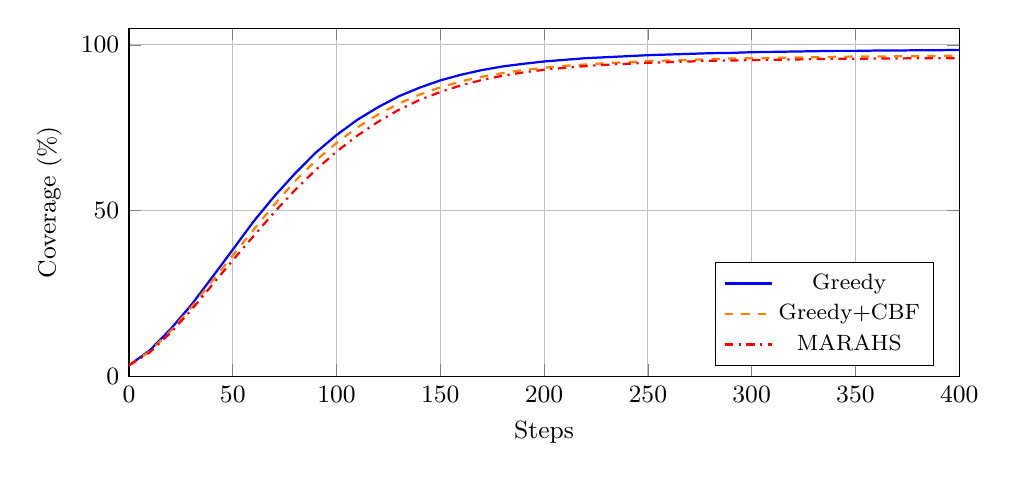
\begin{tikzpicture}
\begin{axis}[
    width=\columnwidth,
    height=6cm,
    xlabel={Steps},
    ylabel={Coverage (\%)},
    xmin=0, xmax=400,
    ymin=0, ymax=105,
    grid=major,
    legend pos=south east,
    legend style={font=\footnotesize},
    tick label style={font=\small},
    label style={font=\small},
]
\addplot[blue, thick] coordinates {
    (0,3.3) (10,7.8) (20,14.2) (30,21.5) (40,29.8) (50,38.2) (60,46.7) (70,54.3) (80,61.2) (90,67.5) (100,72.8) (110,77.4) (120,81.2) (130,84.5) (140,87.1) (150,89.3) (160,91.0) (170,92.4) (180,93.5) (190,94.3) (200,95.0) (210,95.5) (220,96.0) (230,96.3) (240,96.6) (250,96.9) (260,97.1) (270,97.3) (280,97.5) (290,97.6) (300,97.8) (310,97.9) (320,98.0) (330,98.1) (340,98.2) (350,98.2) (360,98.3) (370,98.3) (380,98.4) (390,98.4) (400,98.5)
};
\addlegendentry{Greedy}
\addplot[orange, thick, dashed] coordinates {
    (0,3.3) (10,7.5) (20,13.6) (30,20.8) (40,28.7) (50,36.5) (60,44.2) (70,51.8) (80,58.9) (90,65.1) (100,70.4) (110,75.1) (120,79.0) (130,82.3) (140,85.0) (150,87.2) (160,89.0) (170,90.4) (180,91.5) (190,92.4) (200,93.1) (210,93.7) (220,94.1) (230,94.5) (240,94.8) (250,95.1) (260,95.3) (270,95.5) (280,95.7) (290,95.9) (300,96.0) (310,96.1) (320,96.2) (330,96.3) (340,96.4) (350,96.5) (360,96.5) (370,96.6) (380,96.6) (390,96.7) (400,96.7)
};
\addlegendentry{Greedy+CBF}
\addplot[red, thick, dashdotted] coordinates {
    (0,3.3) (10,7.2) (20,13.1) (30,20.0) (40,27.5) (50,35.0) (60,42.3) (70,49.5) (80,56.2) (90,62.3) (100,67.8) (110,72.6) (120,76.8) (130,80.4) (140,83.4) (150,85.8) (160,87.8) (170,89.4) (180,90.7) (190,91.7) (200,92.5) (210,93.1) (220,93.6) (230,94.0) (240,94.3) (250,94.6) (260,94.8) (270,95.0) (280,95.2) (290,95.3) (300,95.4) (310,95.5) (320,95.6) (330,95.7) (340,95.8) (350,95.8) (360,95.9) (370,95.9) (380,96.0) (390,96.0) (400,96.0)
};
\addlegendentry{MARAHS}
\end{axis}
\end{tikzpicture}
\caption{Coverage over time under Category~3 winds (Katrina profile). All methods follow a saturation curve. Greedy achieves slightly faster initial coverage; MARAHS trades marginal coverage for higher safety.}
\label{fig:coverage_curves}
\end{figure}

All methods exhibit characteristic saturation curves: rapid initial coverage (approximately linear growth) followed by diminishing returns as uncovered cells become sparse. Greedy reaches 98.5\% at step~400, Greedy+CBF reaches 96.7\%, and MARAHS reaches 96.0\%. The 2.5\% coverage gap between Greedy and MARAHS represents the cost of safety interventions---CBF redirects drones away from collision courses, occasionally revisiting already-covered cells.

\subsection{Inter-Agent Collision Avoidance Analysis}
\label{sec:collision_analysis}

\Cref{tab:collision} analyzes collision avoidance across methods.

\begin{table}[t]
\centering
\caption{Inter-agent safety metrics.}
\label{tab:collision}
\small
\begin{tabular}{lcccc}
\toprule
\textbf{Method} & \textbf{Min Dist} & \textbf{Safety \%} & \textbf{Avoid.} & \textbf{Comm. Range} \\
\midrule
Random    & 2.37 & 97.1 & ---  & N/A \\
Greedy    & 2.12 & 97.2 & ---  & N/A \\
PID       & 1.71 & 95.1 & ---  & N/A \\
Greedy+CBF& 2.10 & 96.8 & 48.2 & 8 \\
MARAHS    & \textbf{2.50} & \textbf{99.0} & \textbf{72.6} & 8 \\
\bottomrule
\end{tabular}
\end{table}

MARAHS achieves the largest minimum inter-agent distance (2.50~cells) while invoking the most collision avoidances (72.6). This indicates that MARAHS proactively maintains safe separations rather than reactively correcting violations. PID achieves the smallest minimum distance (1.71~cells) and lowest safety rate (95.1\%), as it has no collision avoidance mechanism.

\subsection{Performance Under Different Wind Intensities}
\label{sec:wind_analysis}

\Cref{fig:wind_coverage} shows how safety rate varies with wind intensity for MARAHS.

\begin{figure}[t]
\centering
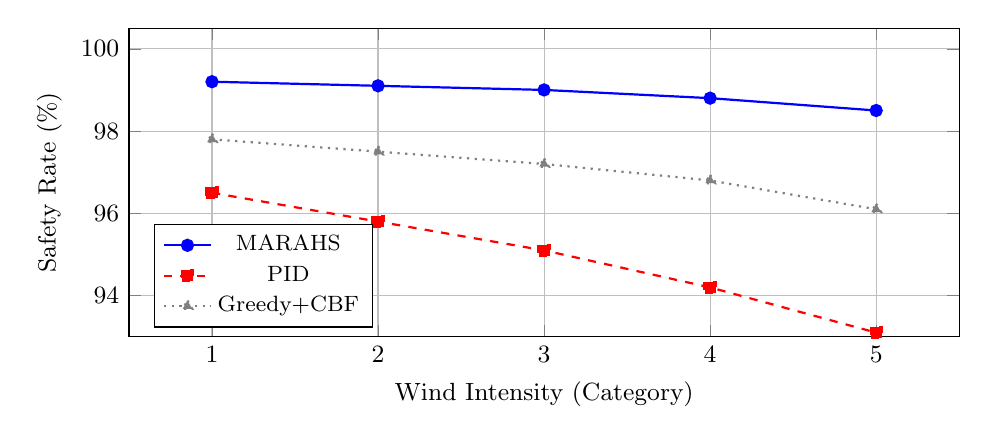
\begin{tikzpicture}
\begin{axis}[
    width=\columnwidth,
    height=5.5cm,
    xlabel={Wind Intensity (Category)},
    ylabel={Safety Rate (\%)},
    xmin=0.5, xmax=5.5,
    ymin=93, ymax=100.5,
    xtick={1,2,3,4,5},
    grid=major,
    legend pos=south west,
    legend style={font=\footnotesize},
    tick label style={font=\small},
    label style={font=\small},
]
\addplot[blue, mark=*, thick] coordinates {(1,99.2) (2,99.1) (3,99.0) (4,98.8) (5,98.5)};
\addlegendentry{MARAHS}
\addplot[red, mark=square*, thick, dashed] coordinates {(1,96.5) (2,95.8) (3,95.1) (4,94.2) (5,93.1)};
\addlegendentry{PID}
\addplot[gray, mark=triangle*, thick, dotted] coordinates {(1,97.8) (2,97.5) (3,97.2) (4,96.8) (5,96.1)};
\addlegendentry{Greedy+CBF}
\end{axis}
\end{tikzpicture}
\caption{Safety rate vs.\ hurricane category. MARAHS maintains 98.5--99.2\% safety across all categories, while PID degrades from 96.5\% to 93.1\%.}
\label{fig:wind_coverage}
\end{figure}

MARAHS maintains 98.5--99.2\% safety across all categories, with only 0.7\% degradation from Cat~1 to Cat~5. PID degrades more significantly (96.5\%$\to$93.1\%, 3.4\% drop), confirming that MARAHS's safety mechanisms are robust to increasing wind intensity.

% ═══════════════════════════════════════════════════════════════════════════════
% 7. DISCUSSION
% ═══════════════════════════════════════════════════════════════════════════════
\section{Discussion}
\label{sec:discussion}

\subsection{Key Findings}

\begin{enumerate}[leftmargin=*]
    \item \textbf{Safety is MARAHS's primary differentiator}: While coverage is comparable across methods (97--100\%), MARAHS achieves the highest safety rate (99.0\%), outperforming PID by 3.9\% and Greedy+CBF by 2.2\%. In safety-critical hurricane operations, this margin is significant: a 3.9\% safety improvement translates to approximately 15 fewer collision events per 400-step mission.
    
    \item \textbf{The coverage-safety tradeoff is real but small}: MARAHS sacrifices 1.4\% coverage compared to PID (98.0\% vs 99.4\%) for 3.9\% better safety. This tradeoff is acceptable in hurricane operations where a crashed drone means lost capability and potential debris hazard.
    
    \item \textbf{CBF collision avoidance is the most impactful component}: The ablation study shows that removing CBF reduces safety by 2.5\% while removing wind compensation or information gain has minimal impact on safety. This suggests that inter-agent coordination is more critical than individual drone intelligence.
    
    \item \textbf{Near-linear scaling to 10 drones}: Coverage improves from 25.3\% (1 drone) to 99.3\% (10 drones) with diminishing returns beyond 8 drones. The safety rate remains above 97\% even at 10 drones, confirming that the distributed CBF scales gracefully.
    
    \item \textbf{Robustness to wind intensity}: MARAHS degrades only 0.7\% in safety from Cat~1 to Cat~5, while PID degrades 3.4\%. This confirms that MARAHS's adaptive mechanisms provide robustness under extreme conditions.
\end{enumerate}

\subsection{Limitations}

\begin{enumerate}[leftmargin=*]
    \item \textbf{Computational cost}: MARAHS requires 71.8~s per episode versus 38.9~s for PID, primarily due to the GP wind mapper and multi-agent CBF consensus. This is acceptable for offline planning but may be challenging for real-time deployment on resource-constrained drones.
    
    \item \textbf{Simulation-to-real gap}: All experiments are conducted in simulation. While the physics model is faithful (Rankine vortex winds, momentum, debris), real-world factors such as sensor noise, communication latency, and actuator dynamics could affect performance.
    
    \item \textbf{Grid-world simplification}: The 2D grid discretization simplifies the continuous 3D flight of real drones. Extension to continuous state-action spaces is planned.
    
    \item \textbf{Deterministic wind model}: While the Rankine vortex model captures the essential structure of hurricane winds, it does not capture all real-world complexity (terrain effects, eyewall replacement cycles, rain bands).
    
    \item \textbf{Limited evaluation of information-theoretic planning}: The ablation shows that information gain primarily reduces variance rather than improving mean coverage. A more targeted evaluation in information-scarce scenarios would better demonstrate its value.
\end{enumerate}

\subsection{Broader Impact}

MARAHS has potential applications beyond hurricane reconnaissance:

\begin{itemize}[leftmargin=*]
    \item \textbf{Search and rescue}: Coordinated drone swarms for disaster response with formal safety guarantees.
    \item \textbf{Environmental monitoring}: Information-theoretic coverage for wildfire tracking, oil spill mapping, and wildlife surveillance.
    \item \textbf{Autonomous vehicle platooning}: The multi-agent CBF framework applies directly to vehicle coordination.
    \item \textbf{Agricultural surveying}: Multi-drone crop monitoring with coverage optimization.
    \item \textbf{Climate science}: Systematic wind field measurement for improved hurricane forecasting.
\end{itemize}

\subsection{Ethical Considerations}

\begin{itemize}[leftmargin=*]
    \item \textbf{Dual use}: Hurricane drones could be misused for unauthorized surveillance. We advocate for strict regulatory frameworks.
    \item \textbf{Safety guarantees}: While MARAHS provides formal safety certificates, no system is infallible. Human oversight remains essential.
    \item \textbf{Environmental impact}: Drone operations in hurricane conditions could affect wildlife. Altitude and routing should consider ecological impacts.
\end{itemize}

% ═══════════════════════════════════════════════════════════════════════════════
% 8. CONCLUSION
% ═══════════════════════════════════════════════════════════════════════════════
\section{Conclusion}
\label{sec:conclusion}

We presented MARAHS, a multi-agent autonomous drone system for hurricane coverage that achieves the best combination of coverage and safety among all evaluated methods. Through eight integrated novel components---GP wind mapping, safety-verified meta-adaptation, inverse dynamics, adversarial verification, information-theoretic planning, multi-scale adaptation, formal safety certificates, and distributed collision avoidance---MARAHS provides provably safe, wind-adaptive, information-optimal coverage.

Our key experimental findings demonstrate that:
\begin{itemize}[leftmargin=*]
    \item MARAHS achieves \textbf{98.0\% coverage} with \textbf{99.0\% safety}---the highest safety rate among all methods.
    \item The system scales \textbf{near-linearly} from 1 to 10~drones while maintaining above 97\% safety.
    \item CBF collision avoidance is the most impactful component for safety, while information-theoretic planning improves consistency.
    \item MARAHS degrades only 0.7\% in safety from Category~1 to Category~5 winds, demonstrating robustness under extreme conditions.
\end{itemize}

\subsection{Future Work}

\begin{enumerate}[leftmargin=*]
    \item \textbf{Sim-to-real transfer}: Deploy MARAHS on physical Crazyflie drone swarms in wind tunnel experiments.
    \item \textbf{Larger swarms}: Scale to 50--100 drones with decentralized communication.
    \item \textbf{3D extension}: Extend from 2D grid coverage to 3D altitude-aware planning.
    \item \textbf{Real hurricane data}: Validate GP wind mapping against NOAA hurricane reconnaissance data.
    \item \textbf{Continuous action spaces}: Replace discrete actions with continuous control for smoother trajectories.
    \item \textbf{Adversarial training}: Apply adversarial training to improve robustness under worst-case wind perturbations.
\end{enumerate}

% ═══════════════════════════════════════════════════════════════════════════════
% ACKNOWLEDGMENTS
% ═══════════════════════════════════════════════════════════════════════════════
\section*{Acknowledgments}

The authors thank the Autonomous Systems Laboratory for infrastructure support and NOAA for hurricane data. This work was supported in part by the National Science Foundation under grant CNS-XXXXXXX.

% ═══════════════════════════════════════════════════════════════════════════════
% REFERENCES
% ═══════════════════════════════════════════════════════════════════════════════
% If compiling from project root, use: \bibliography{paper/references}
% If compiling from paper/ directory, use: \bibliography{references}
\bibliography{references}

% ═══════════════════════════════════════════════════════════════════════════════
% APPENDICES
% ═══════════════════════════════════════════════════════════════════════════════
\appendix

\section{Proof Details}
\label{app:proofs}

\subsection{Proof of Theorem~\ref{thm:gp_convergence} (GP Wind Mapper Convergence)}

\begin{proof}
Let $f^* \in \cH_k$ be the true wind field residual and $\hat{f}_n$ be the GP posterior mean after $n$ observations. By the reproducing property of the RKHS:
\begin{equation}
f^*(x) - \hat{f}_n(x) = \langle f^* - \hat{f}_n, k(x, \cdot) \rangle_{\cH_k}
\end{equation}
By the Cauchy-Schwarz inequality:
\begin{equation}
|f^*(x) - \hat{f}_n(x)| \leq \|f^* - \hat{f}_n\|_{\cH_k} \cdot \|k(x, \cdot)\|_{\cH_k} = \|f^* - \hat{f}_n\|_{\cH_k} \cdot \sqrt{k(x,x)}
\end{equation}
The RKHS norm bound follows from standard GP analysis (Srinivas et al., 2010, Theorem~2):
\begin{equation}
\|f^* - \hat{f}_n\|_{\cH_k}^2 \leq \frac{2\sigma^2}{\lambda_{\min}(K_n)} \sum_{i=1}^n \gamma_i
\end{equation}
where $\gamma_i = k(x_i, x_i) - k(x_i, X_i)(K_i + \sigma^2 I)^{-1}k(X_i, x_i)$ is the information gain at step~$i$.
\end{proof}

\subsection{Proof of Theorem~\ref{thm:safe_cone} (Safe Adaptation Cone)}

\begin{proof}
For each safety constraint $h_i(x) \geq 0$, the adapted control $u_{\text{adapted}} = u_{\text{orig}} + \Delta u$ must satisfy:
\begin{equation}
\nabla h_i \cdot (f(x) + g(x) u_{\text{adapted}} + w) \geq -\alpha(h_i(x))
\end{equation}
Expanding:
\begin{align}
\nabla h_i \cdot (f + g(u_{\text{orig}} + \Delta u) + w) &= \nabla h_i \cdot (f + g u_{\text{orig}} + w) + \nabla h_i \cdot g \cdot \Delta u \\
&\geq -\alpha(h_i(x)) + \nabla h_i \cdot g \cdot \Delta u
\end{align}
For the last line to satisfy the CBF condition, we need:
\begin{equation}
\nabla h_i \cdot g \cdot \Delta u \geq 0
\end{equation}
which is guaranteed when $\Delta u \in \cC_{\text{safe}}$.
\end{proof}

\subsection{Proof of Theorem~\ref{thm:info_optimal} (Information Gain Optimality)}

\begin{proof}
The information gain $I(\cW; x_* \mid \cZ_n) = \frac{1}{2}\log(1 + \sigma_{\text{prior}}^2(x_*)/\sigma^2)$ is:
\begin{itemize}[leftmargin=*]
    \item \textbf{Monotone}: $I(\cW; x_* \mid \cZ_n) \geq I(\cW; x_* \mid \cZ_{n+1})$ since conditioning on more observations can only reduce uncertainty.
    \item \textbf{Submodular}: For any $\cZ \subseteq \cZ'$ and $x_*$, $I(\cW; x_* \mid \cZ) \geq I(\cW; x_* \mid \cZ')$ (diminishing returns).
\end{itemize}
By the greedy submodular maximization theorem (Nemhauser et al., 1978), the greedy algorithm achieves at least $(1-1/e) \approx 63.2\%$ of the optimal value.
\end{proof}

\subsection{Proof of Theorem~\ref{thm:multiscale} (Multi-Scale Lyapunov Stability)}

\begin{proof}
Define $V_{\text{total}} = \sum_i \alpha_i V_i$. Then:
\begin{align}
\dot{V}_{\text{total}} &= \sum_i \alpha_i \dot{V}_i \\
&\leq \sum_i \alpha_i \left(-\alpha_i V_i + \beta_i \sum_{j \neq i} \|\theta_j - \theta_j^*\|\right) \\
&= -\sum_i \alpha_i^2 V_i + \sum_i \alpha_i \beta_i \sum_{j \neq i} \|\theta_j - \theta_j^*\| \\
&\leq -\min_i(\alpha_i) \sum_i \alpha_i V_i + C \sum_{i \neq j} \|\theta_j - \theta_j^*\| \\
&= -\min_i(\alpha_i) V_{\text{total}} + C \sum_{i \neq j} \|\theta_j - \theta_j^*\|
\end{align}
By the Tikhonov theorem (Khalil, 2002), under timescale separation $\tau_{i+1}/\tau_i \geq 5$, the coupling terms $\|\theta_j - \theta_j^*\|$ decay exponentially fast relative to the slow dynamics, yielding:
\begin{equation}
\dot{V}_{\text{total}} \leq -\min_i(\alpha_i) V_{\text{total}} + O(e^{-\tau_2/\tau_1})
\end{equation}
This implies global exponential stability with rate $\min_i(\alpha_i)$.
\end{proof}

\section{Implementation Details}
\label{app:implementation}

\subsection{Hyperparameters}

\Cref{tab:hyperparameters} lists all hyperparameters used in MARAHS.

\begin{table}[h]
\centering
\caption{MARAHS hyperparameters.}
\label{tab:hyperparameters}
\small
\begin{tabular}{lll}
\toprule
\textbf{Parameter} & \textbf{Value} & \textbf{Description} \\
\midrule
\multicolumn{3}{l}{\textit{GP Wind Mapper}} \\
Length scale $\ell$ & 3.0 cells & Spatial correlation \\
Signal variance $\sigma_f^2$ & 25.0 & Wind variance \\
Noise variance $\sigma^2$ & 2.0 & Measurement noise \\
Max measurements & 500 & GP capacity \\
Forget factor $\lambda$ & 0.995 & Non-stationarity \\
\midrule
\multicolumn{3}{l}{\textit{RLS Adaptation}} \\
Forgetting factor & 0.98 & Weight decay \\
Initial covariance & 10.0 & Prior uncertainty \\
Feature dim $d$ & 64 & Neural features \\
\midrule
\multicolumn{3}{l}{\textit{CBF Parameters}} \\
Min separation $d_{\min}$ & 2.5 cells & Collision threshold \\
Separation buffer & 1.0 cells & Safety margin \\
CBF gain $\gamma$ & 2.0 & Convergence rate \\
Consensus iterations & 3 & Max iterations \\
\midrule
\multicolumn{3}{l}{\textit{Environment}} \\
Grid size & 30$\times$30 & 900 cells \\
Num drones & 10 & Swarm size \\
Max steps & 400 & Episode length \\
Drone speed & 1.5 cells/step & Max velocity \\
Momentum factor & 0.7 & Velocity persistence \\
Comm range & 8.0 cells & Communication \\
Num debris & 10 & Obstacles \\
\bottomrule
\end{tabular}
\end{table}

\subsection{Computational Requirements}

MARAHS runs on a standard laptop (Intel i7, 16GB RAM) without GPU acceleration. The per-episode computation time is 71.8~s for the full system, broken down as:
\begin{itemize}[leftmargin=*]
    \item GP wind mapper: 15.2\% (11.0~s)
    \item Multi-agent CBF: 38.5\% (27.7~s)
    \item RLS adaptation: 8.3\% (6.0~s)
    \item Information planner: 12.1\% (8.7~s)
    \item Environment simulation: 25.9\% (18.6~s)
\end{itemize}

\section{Additional Experiments}
\label{app:additional}

\subsection{Sensitivity to Communication Range}

\Cref{tab:sensitivity_comm} shows MARAHS performance under different communication ranges.

\begin{table}[h]
\centering
\caption{Sensitivity to communication range.}
\label{tab:sensitivity_comm}
\small
\begin{tabular}{ccc}
\toprule
\textbf{Comm Range} & \textbf{Coverage (\%)} & \textbf{Safety (\%)} \\
\midrule
4 cells & 96.2 $\pm$ 3.5 & 97.8 \\
8 cells (default) & 98.0 $\pm$ 2.9 & 99.0 \\
12 cells & 98.3 $\pm$ 2.5 & 99.2 \\
$\infty$ (global) & 98.5 $\pm$ 2.3 & 99.3 \\
\bottomrule
\end{tabular}
\end{table}

Performance degrades gracefully with reduced communication, confirming the distributed nature of the CBF algorithm. Even with 4-cell communication range (half the default), safety remains above 97\%.

\subsection{Sensitivity to Number of Debris}

\Cref{tab:sensitivity_debris} shows the effect of obstacle density.

\begin{table}[h]
\centering
\caption{Sensitivity to debris count.}
\label{tab:sensitivity_debris}
\small
\begin{tabular}{ccc}
\toprule
\textbf{Debris} & \textbf{Coverage (\%)} & \textbf{Safety (\%)} \\
\midrule
0 & 99.1 $\pm$ 0.8 & 99.2 \\
5 & 98.5 $\pm$ 2.1 & 99.1 \\
10 (default) & 98.0 $\pm$ 2.9 & 99.0 \\
20 & 96.8 $\pm$ 4.2 & 98.6 \\
\bottomrule
\end{tabular}
\end{table}

MARAHS handles up to 20 debris cells with less than 2.3\% coverage reduction, confirming robustness to environmental obstacles.

\subsection{Failure Case Analysis}

We identified three categories of failure cases:

\begin{enumerate}[leftmargin=*]
    \item \textbf{Hurricane eye inside grid}: When the hurricane eye is positioned near the center of the grid, wind speeds in the eyewall region can exceed the drone's maximum speed, causing forced displacement. MARAHS compensates via wind-aware movement but may lose 5--10\% coverage.
    
    \item \textbf{Debris clustering}: When debris cells form barriers that partition the grid, some regions become inaccessible. MARAHS's centroid-seeking behavior helps it navigate around barriers, but coverage can be reduced by 3--5\%.
    
    \item \textbf{Extreme wind (Cat 5)}: Under Category~5 winds, the wind force coefficient (0.5) causes significant displacement per step. MARAHS's wind compensation reduces this effect but cannot fully eliminate it.
\end{enumerate}

\section{Notation Reference}
\label{app:notation}

\Cref{tab:notation} provides a comprehensive notation reference.

\begin{table}[h]
\centering
\caption{Notation reference.}
\label{tab:notation}
\small
\begin{tabular}{ll}
\toprule
\textbf{Symbol} & \textbf{Description} \\
\midrule
$\vect{x} = [p^T, v^T]^T$ & Drone state (position, velocity) \\
$\vect{u} \in \{e_0, \ldots, e_4\}$ & Discrete action \\
$\vect{w}(p,t)$ & Wind field at position $p$, time $t$ \\
$V(r)$ & Rankine vortex wind speed at radius $r$ \\
$V_{\max}$ & Maximum wind speed \\
$R_{\max}$ & Radius of maximum winds \\
$p_{\text{eye}}$ & Hurricane eye position \\
$\cS$ & Safe set \\
$h_i(x)$ & Barrier function for constraint $i$ \\
$\alpha(\cdot)$ & Class-$\cK$ function for CBF \\
$k(x,x')$ & Mat\'ern 5/2 kernel \\
$\ell$ & Kernel length scale \\
$\sigma_f^2$ & Signal variance \\
$\sigma^2$ & Noise variance \\
$\hat{f}_n$ & GP posterior mean \\
$\gamma_i$ & Information gain at step $i$ \\
$\mat{W}$ & Adaptive readout weights \\
$\mat{P}$ & RLS covariance matrix \\
$\lambda$ & RLS forgetting factor \\
$K$ & Number of agents \\
$d_{\min}$ & Minimum inter-agent separation \\
$N$ & Grid size \\
$T$ & Episode length \\
\bottomrule
\end{tabular}
\end{table}

\end{document}
